%\usepackage[utf8x]{inputenc}
%\usepackage{fancyhdr}
%\pagestyle{fancy}

\chapter{Seismology}
\newpage
\subsection{Seismic Cycle}
Earthquakes triggering is a complex mechanism. However, it is the same
mechanisms that generate millimeter or multi-kilometer ruptures. 

During the \textbf{interseismic stage}, which makes up most of the cycle, a
loading (e.g. a force accumulation) occurs on asperities locating on the shallow
part of the fault. This part is "locked", although some deformations affect the
deeper part of the fault via a aseismic creep (figure
\ref{figure_seismic_cycle}b). 

After a long period of time, the rock failure threshold $\sigma_c$ on an
asperity is reached, the rock break and a slip begin at this point. This phase,
the \textbf{coseismic stage}, lasts few second to minutes and meters of slip on
the fault "catch up" with the few mm/yr of motion that occurred during the
interseismic stage (figure \ref{figure_seismic_cycle}c). This quick emission of
energy generates seismic waves and unloads the asperities on a quantity called
"stress drop" ($\Delta \sigma$).  When the energy released become too low to
propagate the rupture, the slip stops and the asperity begin again to accumulate
stresses.

Finally, a \textbf{postseismic stage} occurs after the earthquake, and
aftershock and transient afterslip occur for a period of years before the fault
settles into its steady interseismic behavior again.
\begin{figure}[h]
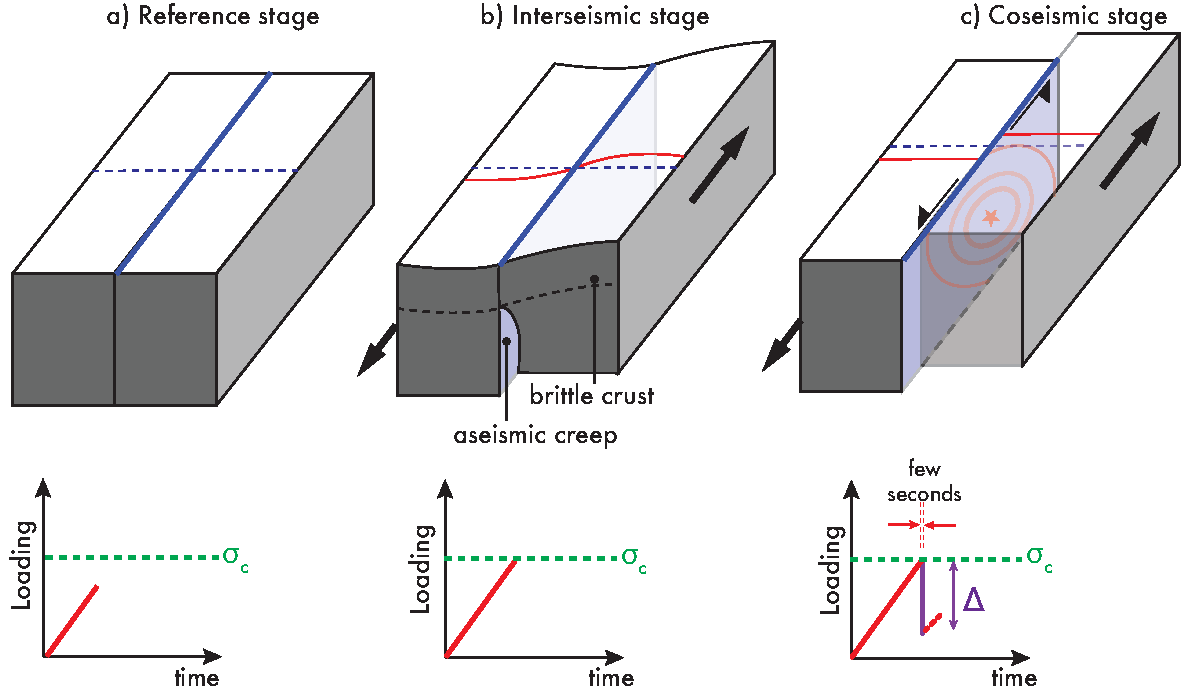
\includegraphics[trim = 5mm 180mm 0mm 0mm, clip,scale=0.6]{seismology/figures/seismic_cycle.pdf}
\caption{From a initial stage (a), a fault accumulates loading on the locked
    part during the interseismic stage (b), and a slowly deformation appears on
    the surface. When the rock failure on the fault is reached, the coseismic
    stage (c) begin and the fault breaks : it's an earthquake birth.}
\label{figure_seismic_cycle}
\end{figure}

These types of deformations can be observed by geodesy. For example, GPS
stations can recorded deformation for some years for specific points on the
surface, and radar interferometry (measuring precisely the displacement between
two pictures of the same areas) can showed the co-seismic effect after an
earthquake (Figure \ref{figure_seismic_cycle_subduction}). 

\begin{figure}[h]
\centering
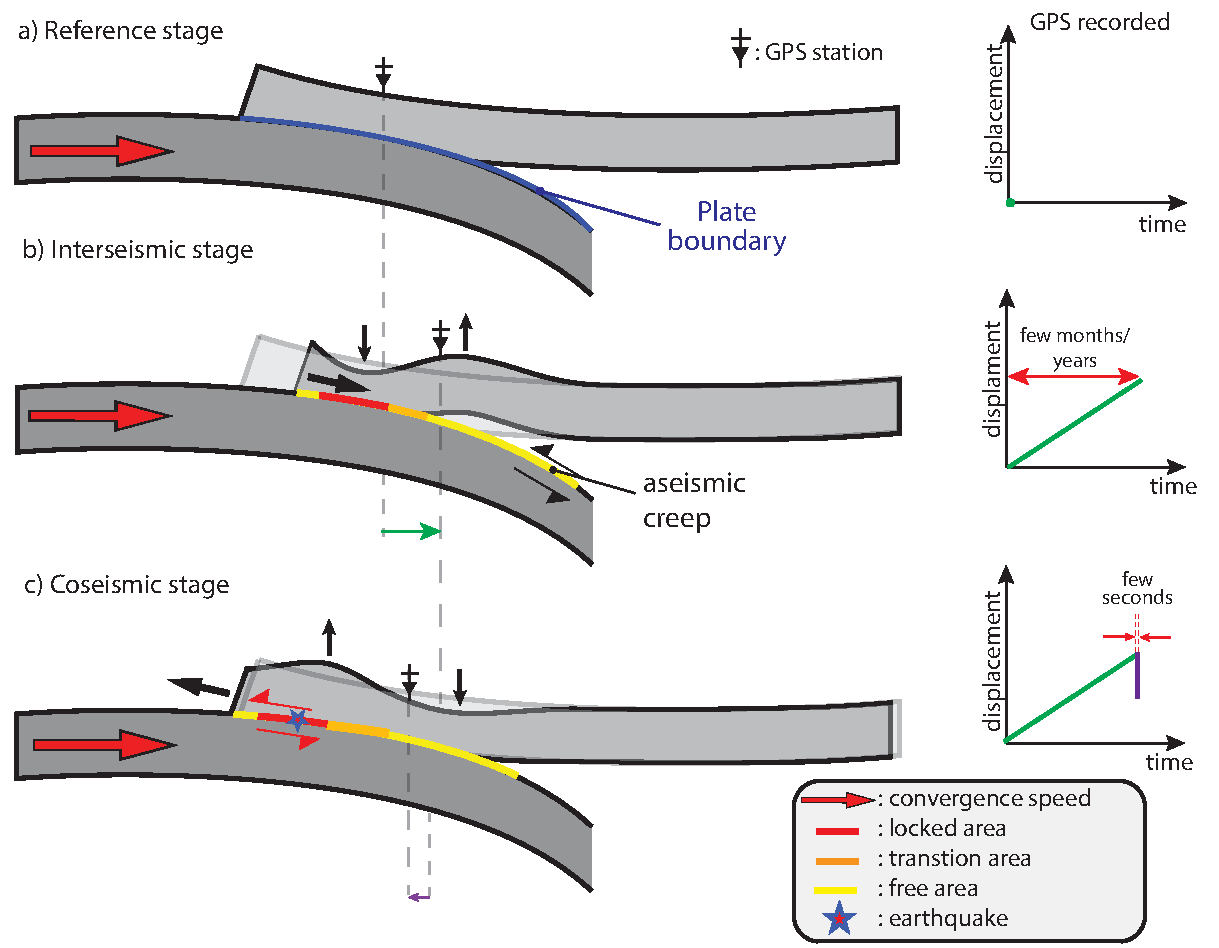
\includegraphics[trim = 5mm 120mm 0mm 0mm, clip,scale=0.5]{seismology/figures/seismic_cycle_subduction.pdf}
\caption{Seismic cycle representation in the subduction context. Displacements can be observed by geodetic method as GPS station. }
\label{figure_seismic_cycle_subduction}
\end{figure}

\subsection{Magnitude}
More the energy released by earthquake is important, more earthquake will be
strong. Indeed, this energy is used to break the rock and spread the rupture. A
common equation to quantify this energy is the \textit{seismic moment} $M_0$:
\begin{equation}
M_0= \mu \times  \bar{d} \times S
\end{equation}
 where $\mu$ is the shear modulus (or modulus of rigidity), $\bar{d}$ is the
 average fault displacement on the fault with area $S$. The unit of the seismic
 moment is N.m (but older references express $M_0$ in dyne-cm).
 
 For historical reasons, the most well-known measure of earthquake size is the
 earthquake magnitude. There are now several different types of magnitude scales
 but all are related to the largest amplitude that is recorded on a seismogram.
 This is one of the easiest things to measure and is one reason for the
 continued popularity of magnitude scales.

The earliest magnitude scale and introduced by Charles Richter in 1935, is the \textit{local magnitude} $M_L$, based on the maximum amplitude $A$ (often S-waves) in micrometers recorded on standard short period (1 sec) seismometer and corrected with a standard value $A_0$ depending of the distance between source and the receiver as:
\begin{equation}
    M_L= \log_{10}(A/A_0)
\end{equation}
This magnitude is correct for earthquakes less than 1000 kilometers from the instrument measuring the earthquake.

But with time, other magnitudes types appeared. The first one is the \textit{body-wave magnitude} $m_b$, based on the measure of the amplitude of the P body waves generated by the earthquake, using:
\begin{equation}
    m_b= \log_{10}(A/T) + Q(D,h)
\end{equation}
where T (in second) is the period of the wave being measured, $A$ is its
amplitude and $Q(D,h)$ is a correction factor that is a function of distance,
$D$ (in degrees), between epicenter and station and focal depth, $h$ (in
kilometers), of the earthquake

The \textit{surface wave magnitude} $M_S$ is measured using the largest amplitude of the surface waves and its general formula is: 
\begin{equation}
    M_S= \log_{10} (A/T) + 1.66 \log_{10} (D) +3.3
\end{equation}

When initially developed, these magnitude scales were considered to be equivalent; in other words, earthquakes of all sizes were thought to radiate fixed proportions of energy at different periods. But it turns out that larger earthquakes, which have larger rupture surfaces, systematically radiate more long-period energy. Thus, for very large earthquakes, body-wave magnitudes badly underestimate true earthquake size; the maximum body-wave magnitudes are about 6.5--6.8. In fact, the surface-wave magnitudes underestimate the size of very large earthquakes; the maximum observed values are about 8.3--8.7.

To avoid these saturation problems, Kanamori in 1977 proposed the \textit{moment magnitude} $M_w$ using the seismic moment $M_0$:
\begin{equation}
    M_w = \frac{2}{3} \log_{10} (M_0) - 6.1
\end{equation}
Now, this final formula is the most commonly magnitude used and it allows to estimate that the energy increase of factor $\times 32$  between a magnitude $M_w$ and $M_w+1$  (Table~\ref{tab:table_Seismic_Energy}).

\begin{table}[h]
    \caption{Examples of values for different historical eathquakes. (from Stein
    and Wysession 2003)}
    \label{tab:table_Seismic_Energy}
    \begin{tabular}{ccccc}
        \toprule 
        \textbf{Earthquake} &
        \textbf{Fault area} (\si{km^2}) &
        \textbf{Average} &
        \textbf{Seismic moment} &
        \textbf{Moment} \\ 
        {} &
        (length $\times$ width) &
        \textbf{Dislocation} (\si{m}) &
        (\si{dyne.cm}), $M_0$ &
        \textbf{Magnitude}, $M_w$ \\ 
        \midrule 
        Truckee, 1966 & 10 $\times$ 10 & 0.3  & $8.3 \times 10^{24}$ & 5.9 \\ 
        San Fernando, 1971 & 20 $\times$ 14 & 1.4  & $1.2 \times 10^{26}$ & 6.7 \\ 
        Loma Prieta, 1989 & 40 $\times$ 15 & 1.7 & $3.0 \times 10^{26}$ & 6.9 \\ 
        San Francisco, 1906 & 450 $\times$ 10& 4 & $5.4 \times 10^{27}$  & 7.8 \\ 
        Alaska, 1964 & 500 $\times$ 300 & 7 & $5.2 \times 10^{29}$ & 9.1 \\ 
        Chile, 1960 & 800 $\times$ 200 & 21 & $2.4 \times 10^{30}$ & 9.5 \\ 
        \bottomrule 
    \end{tabular} 
\end{table}

\subsection{Earthquake statistics}
\subsubsection{Relation between magnitude and frequency}
If you look at the number of earthquake per magnitude for a specific region and for a period of time,  you can observe that the number of events of low magnitudes is more important than for high magnitude. This observation was quantified by Gutenberg and Richter in the 1940s via the following relation known as the \textit{Gutenberg and Richter law}:
\begin{equation}
    \log_{10} N=  a - b \times M
\end{equation}
where $N$ is the number of earthquakes with magnitude greater than $M$ occurring in a given time, $a$ depends on the number of earthquakes in the time and region sampled and the slope $b$ is generally about 1 (Figure~\ref{fig:figure_GR_law}).

\begin{figure}[h]
    \centering
    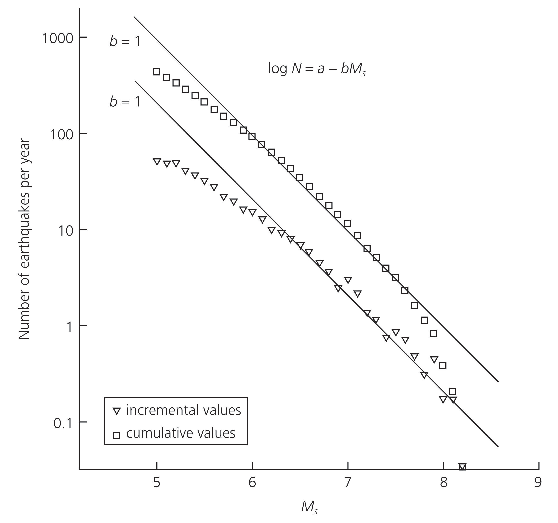
\includegraphics[trim = 0mm 0mm 0mm 4mm, clip,scale=0.9]{seismology/figures/4_7_01.pdf} \caption{Frequency-magnitude plot for all earthquakes with $M_S \geqslant 5.0$ during 1968-97 listed in the catalog of the National Earthquake Information Center (from Stein and Wysession 2003).}
    \label{fig:figure_GR_law}
\end{figure}

\subsubsection{Aftershocks distribution}
After an earthquake occurrence (called mainshock), following events triggered by this earthquake, (called aftershocks) have a characteristic distribution in size and time. The largest aftershocks are usually more than a magnitude unit smaller than the mainshock, and the size distribution is agreed with the Gutenberg-Richter law, although the energy released by the aftershock is usually less than 10 $\%$ of that the mainshock.

Most of the aftershocks occur after the mainshock, and the number of events $n(t)$ is described by the relation:
\begin{equation}
    n(t) =  \frac{K}{(t+c)^p}
\end{equation}
where $p$ is typically about 1, $K$ is the productivity parameter and $c$ is a constant. This law is called the Omori-Utsu law and can be observed after any earthquake (Figure~\ref{fig:aftershock_distribution}).
\begin{figure}[h]
    \centering
    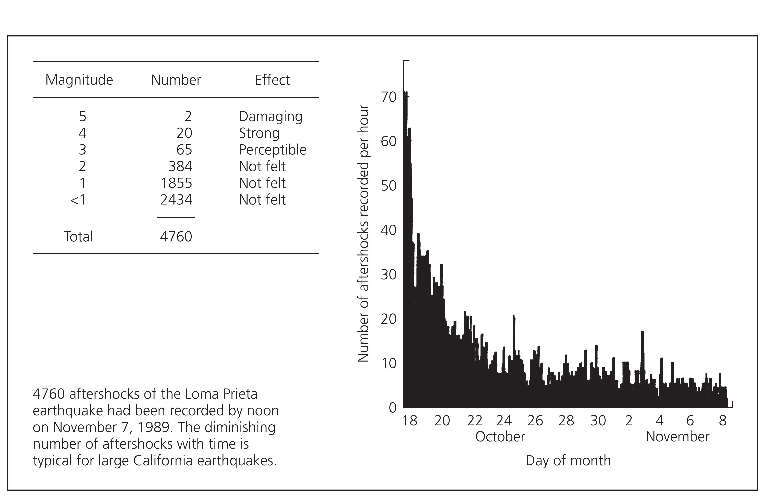
\includegraphics[trim = 2mm 2mm 2mm 8mm, clip,scale=1]{seismology/figures/4_7_08.pdf}
    \caption{Graphic showing the number and distribution aftershock in 22 days after the 1989 Loma Prieta earthquake as functions of magnitude and time (from Stein and Wysession 2003).}
    \label{fig:aftershock_distribution}
\end{figure}

It is important to know that the Earth is perpetually close to the rupture and small stress variations can trigger earthquakes.  A mainshock occurrence perturbs the stress for a specific region, and more the mainshock is important, more the perturbed region will be spread. A first perturbation mechanism is due to the dynamic stress variations produced by the seismic waves of the mainshock.  This phenomenon allows to explain aftershock occurrences in far field.  The other mechanism is called the static stress variations and corresponds to the variations due to the coseismic displacement. The coseismic displacements change the shear and normal stresses for faults present in the perturbed region by mainshock.  These variations of shear stress ($\Delta \tau_s$) and normal stress ($\Delta \sigma_n$) allows to estimate a parameter called the Coulomb stress changes ($\Delta CFF$) with the equation:
\begin{equation}
    \Delta CFF = \Delta \tau_s + \mu' \Delta \sigma_n
\end{equation} where $\mu'$ is the
effective coefficient of friction. This value of $\Delta CFF$ can be positive or negative and not really high (usually less than 1 bar only) but consistent observations between the region where the $\Delta  CFF$ is positive and the aftershocks locations were observed is some cases (as in 1992 Landers earthquake, in California, see Figure~\ref{fig:Coulomb_map}).
\begin{figure}[h!]
    \centering
    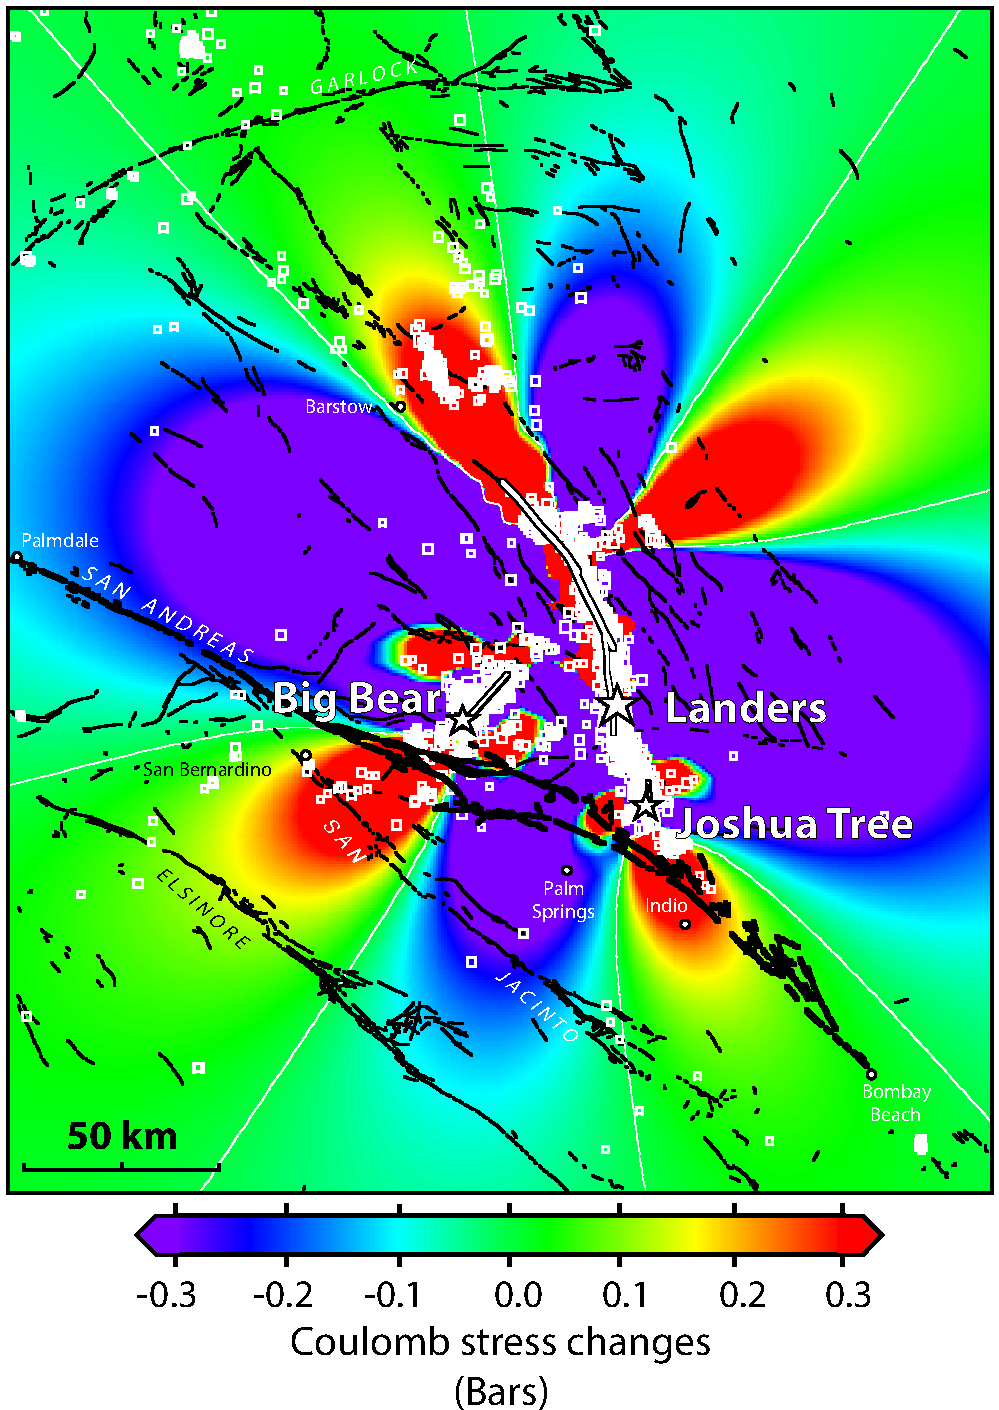
\includegraphics[trim = 25mm 10mm 23mm 20mm,
    clip,scale=0.5]{seismology/figures/Coulomb_Landers.pdf}
    \caption{Map of Coulomb stress changes after the occurrence of Joshua Tree, Landers and Big Bear earthquake. White squares indicate locations of aftershocks (from King et al, 1994). }
    \label{fig:figure_Coulomb_map}
\end{figure}

